%%%simulacion
\chapter{Resultados}

\section{Introducci\'{o}n}

Uno de los objetivos principales de este trabajo consiste en la implementaci\'{o}n pr\'{a}ctica del algoritmo de estabilizaci\'{o}n por modos deslizantes propuesto adem\'{a}s de su comparaci\'{o}n cuantitativa con un algoritmo de control basado en un compensador proporcional-integral el cual es ampliamente usado para el control de este tipo de sistemas. En el cap\'{i}tulo~\ref{sec:ControlChapter} se obtuvieron resultados de simulaci\'{o}n sobre la efectividad del algoritmo de estabilizaci\'{o}n, sin embargo para poder comprobar de una forma m\'{a}s completa el algoritmo es necesaria una implementaci\'{o}n pr\'{a}ctica. Para poder obtener datos sobre el comportamiento del sistema dise\~{n}ado frente a las perturbaciones, se utiliz\'{o} una unidad de medici\'{o}n inercial para la medici\'{o}n de las perturbaciones introducidas en el sistema, este sensor se monta en la base del gimbal y las perturbaciones se realizan de forma manual al manipular el gimbal tratando de ser consistente en los movimientos que se realizan en cada experimento. Las pruebas se realizan de esta manera ya que el dise\~{n}o y construcci\'{o}n de una plataforma de pruebas actuada y con un sistema de control esta fuera del alcance de este trabajo.



\section{Descripci\'{o}n de la Experimentaci\'{o}n}

Para la obtenci\'{o}n de los resultados se realizaron varios experimentos, en los cuales se mont\'{o} una Unidad de Medici\'{o}n Inercial (IMU por sus siglas en ingl\'{e}s) en la base del sistema gimbal, que nos permite medir las perturbaciones inducidas en el sistema, es decir, las velocidades angulares $\omega _{B_y}$ y $\omega _{B_z}$. La IMU utilizada es la MicroStrain 3DM-GX3-25-OEM, que nos permiti\'{o} obtener los datos de la velocidad angular a una frecuencia de 100 Hz en la computadora por medio del software MIP\textsuperscript{\textregistered} Monitor para el control de la IMU, en la figura ~\ref{fig:Prueba} podemos observar la recepci\'{o}n de los datos provenientes de la IMU en la computadora.   

\begin{figure}[H]
\centering
      \includegraphics[scale=0.09]{img/Experimentacion.jpg}
      \caption{Pruebas Experimentales}
      \label{fig:Prueba}
\end{figure}

Los datos obtenidos de las velocidades angulares en la base del sistema se guardan en un archivo para poder ser analizados posteriormente y comparados con los datos obtenidos de la IMU montada en el eslab\'{o}n interno del gimbal. El sistema fue perturbado de forma manual enfatizando las perturbaciones en los ejes $y$ y $z$ del sistema, ya que estos son los de mayor inter\'{e}s al ser los ejes actuados. \'{E}sta metodolog\'{i}a se llev\'{o} a cabo para el algoritmo por modos deslizantes y para el compensador PI para poder observar ambas respuestas, a continuaci\'{o}n se presentan los resultados. 

%\begin{figure}[H]
%\centering
%      \includegraphics[scale=0.5]{img/MicroStrain.jpg}
%      \caption{Unidad de Medici\'{o}n Inercial MicroStrain}
%      \label{fig:MicroStrain}
%\end{figure}

\section{Resultados Algoritmo Proporcional-Integral}  

En la figura ~\ref{fig:ResPIPer}-a podemos observar la perturbaci\'{o}n ejercida sobre el sistema, mientras que en la figura ~\ref{fig:ResPIPer}-b se muestra la velocidad angular medida en el eslab\'{o}n interno del gimbal, es decir, la respuesta del sistema con el algoritmo del compensador Proporcional-Integral programado en las tarjetas de control. 

\begin{figure}[H]
\centering 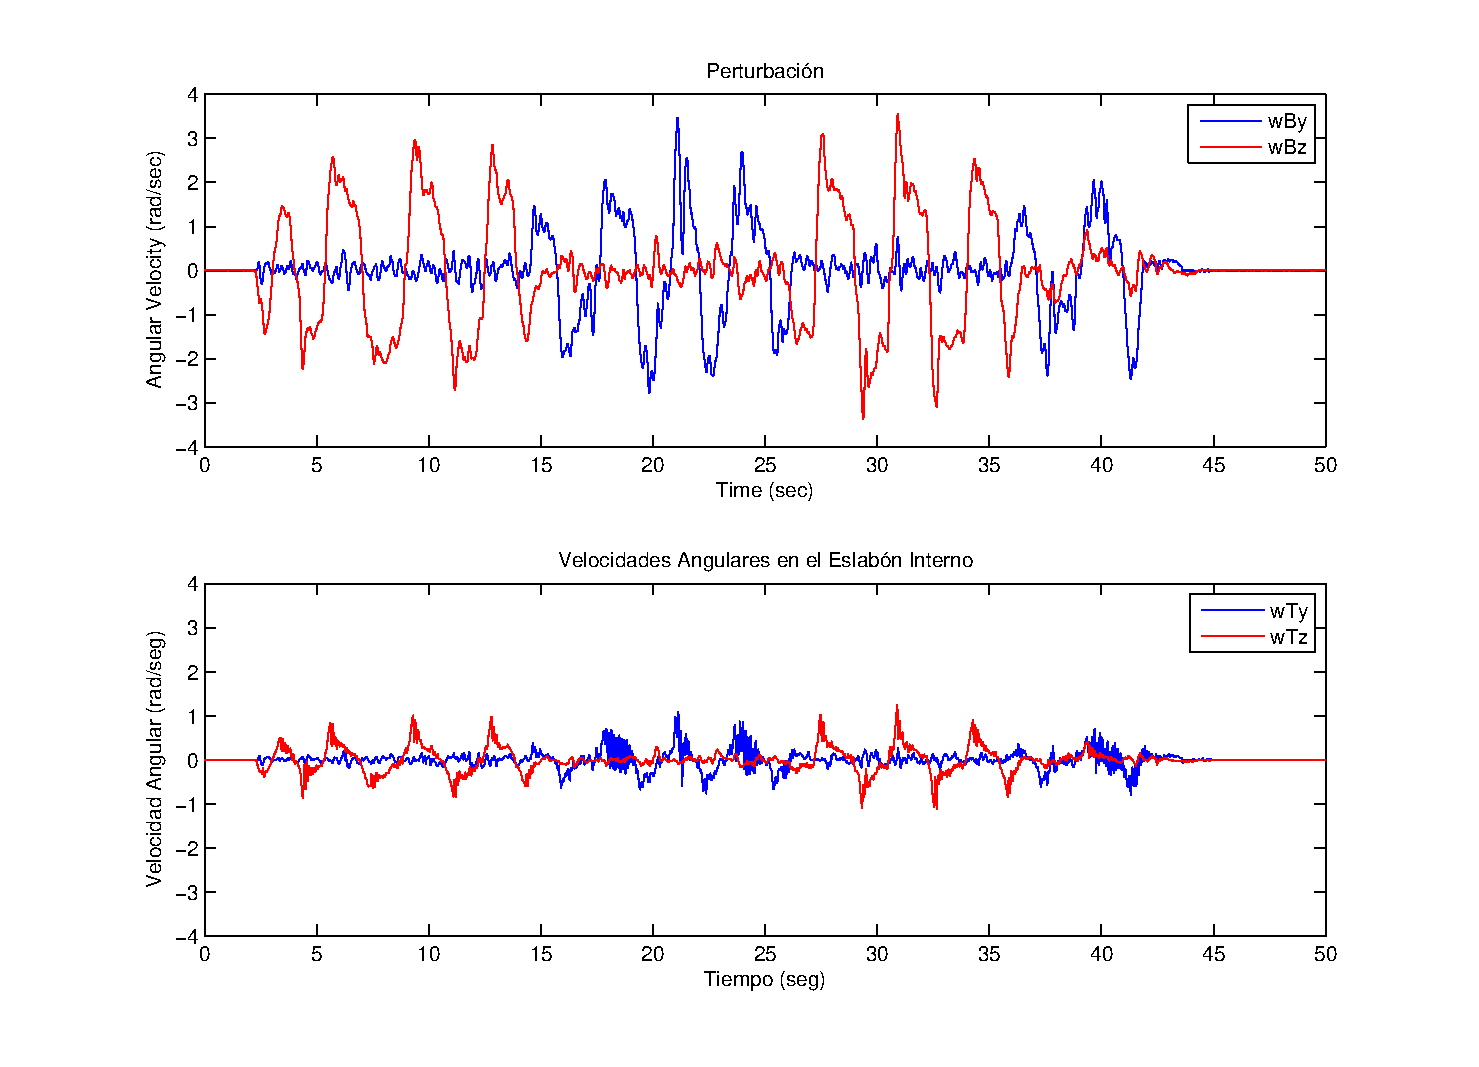
\includegraphics[scale=0.63,trim = 20mm 0mm 20mm 0mm]{img/ResPIPer.eps}
%trim = izquierda abajo derecha arriba [scale=0.5,trim = 40mm 30mm 110mm 15mm, clip]
      \caption{Resultados de la Estabilizaci\'{o}n Proporcional-Integral}
      \label{fig:ResPIPer}
\end{figure}

Podemos observar que el algoritmo compensa en gran medida las perturbaciones, sin embargo la estabilizaci\'{o}n no es perfecta, esto puede deberse a varios factores , por ejemplo la sintonizaci\'{o}n de las constantes de control $K_p$ y $K_i$ podr\'{i}a no ser la \'{o}ptima, ecuaciones ~\ref{eq:ContPIElev} y ~\ref{eq:ContPICross}, adem\'{a}s el algoritmo de estabilizaci\'{o}n se ejecuta en la tarjeta de control a una frecuencia de 40 Hz la cual es posible que no sea suficiente para eliminar las perturbaciones aplicadas.  

En la figura ~\ref{fig:ResPIVs}-a se muestra la comparaci\'{o}n entre la perturbaci\'{o}n aplicada en el eje-$y$, $\omega_{B_y}$ y la velocidad angular sobre el eje de elevaci\'{o}n $\omega_{T_y}$. En la figura ~\ref{fig:ResPIVs}-b, se muestra la perturbaci\'{o}n al sistema $\omega_{B_z}$ gr\'{a}ficada junto con la velocidad angular del gimbal en el eje de la elevaci\'{o}n cruzada $\omega_{T_z}$. 

\begin{figure}[H]
\centering 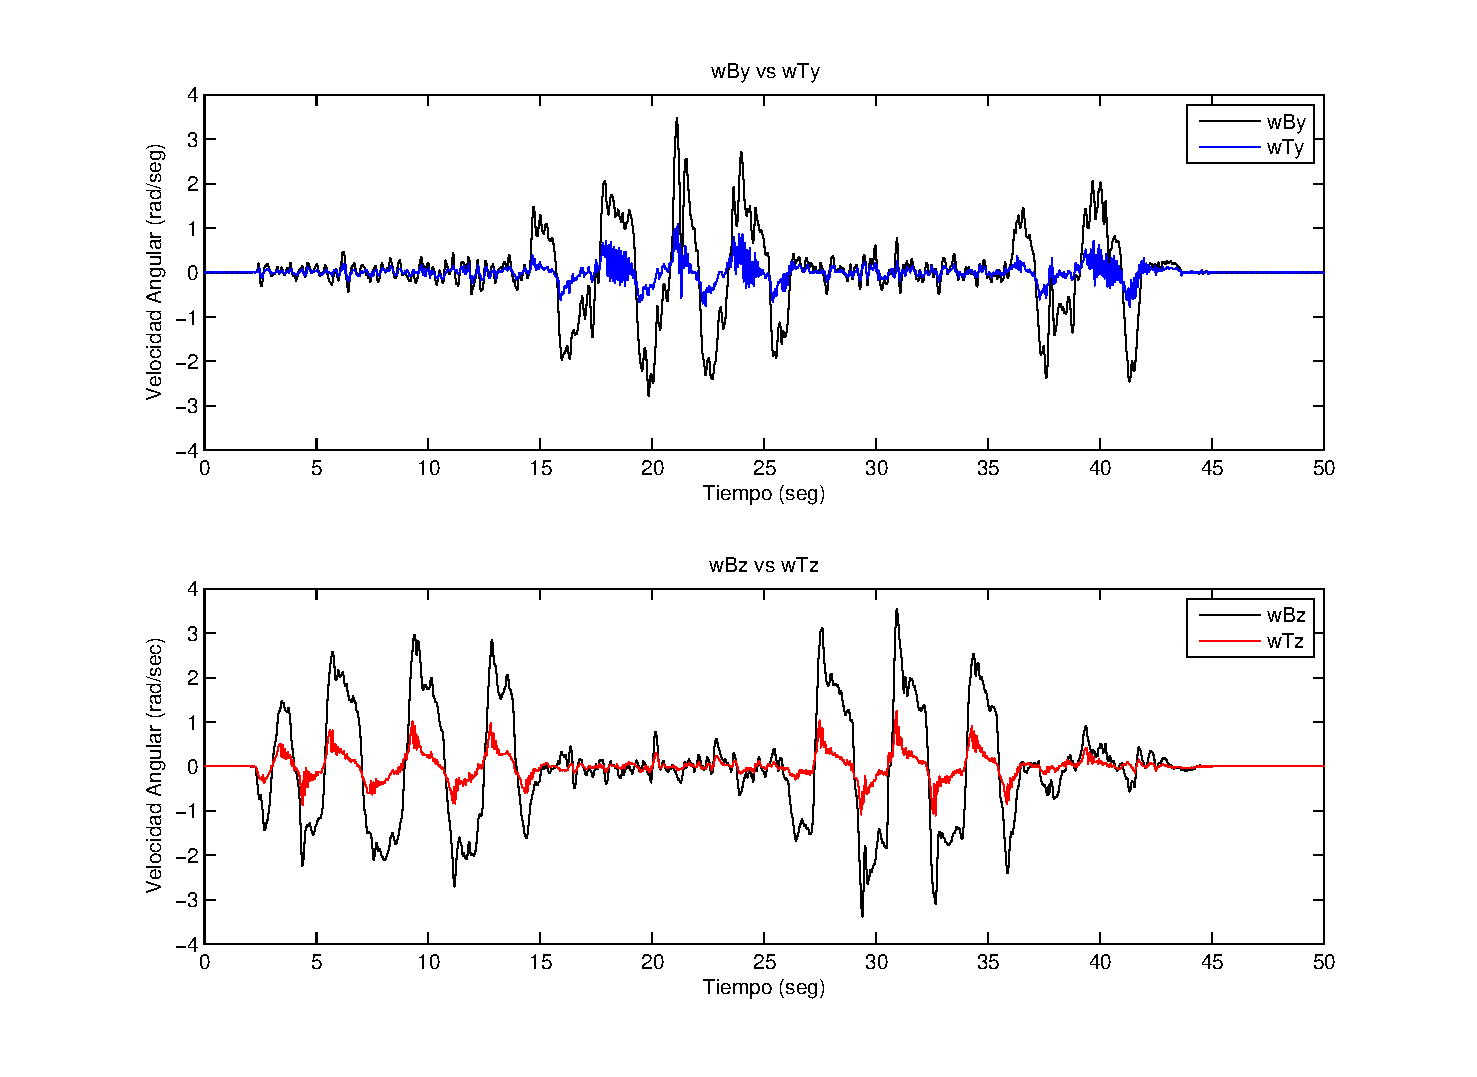
\includegraphics[scale=0.63,trim = 20mm 0mm 20mm 0mm]{img/ResPIVs.eps}
%trim = izquierda abajo derecha arriba [scale=0.5,trim = 40mm 30mm 110mm 15mm, clip]
      \caption{Resultados de la Estabilizaci\'{o}n Proporcional-Integral}
      \label{fig:ResPIVs}
\end{figure}

Estas g\'{a}ficas nos permiten observar m\'{a}s detalladamente el efecto de la estabilizaci\'{o}n sobre los ejes de inter\'{e}s, estas nos muestran la perturbaci\'{o}n ejercida sobre el sistema en contraste con la acci\'{o}n de control. Podemos ver que el algoritmo de control reduce las perturbaciones, logrando en parte el objetivo de estabilizar la l\'{i}nea de vista de la c\'{a}mara montada en el eslab\'{o}n interno del gimbal.

\section{Resultados Algoritmo Por Modos Deslizantes}

En esta secci\'{o}n se exponen los resultados obtenidos de la implementaci\'{o}n del algoritmo de estabilizaci\'{o}n por modos deslizantes en el prototipo construido. De igual forma que para el compensador PI, se perturb\'{o} el sistema de manera manual. En la figura ~\ref{fig:ResSMPer}-a se muestran las gr\'{a}ficas de las perturbaciones medidas por la IMU Microstrain montada en la base del sistema. En la figura ~\ref{fig:ResSMVs}-b se muestra la velocidad angular medida en los ejes de inter\'{e}s de elevaci\'{o}n y elevaci\'{o}n cruzada ante las perturbaciones ejercidas.   

\begin{figure}[H]
\centering 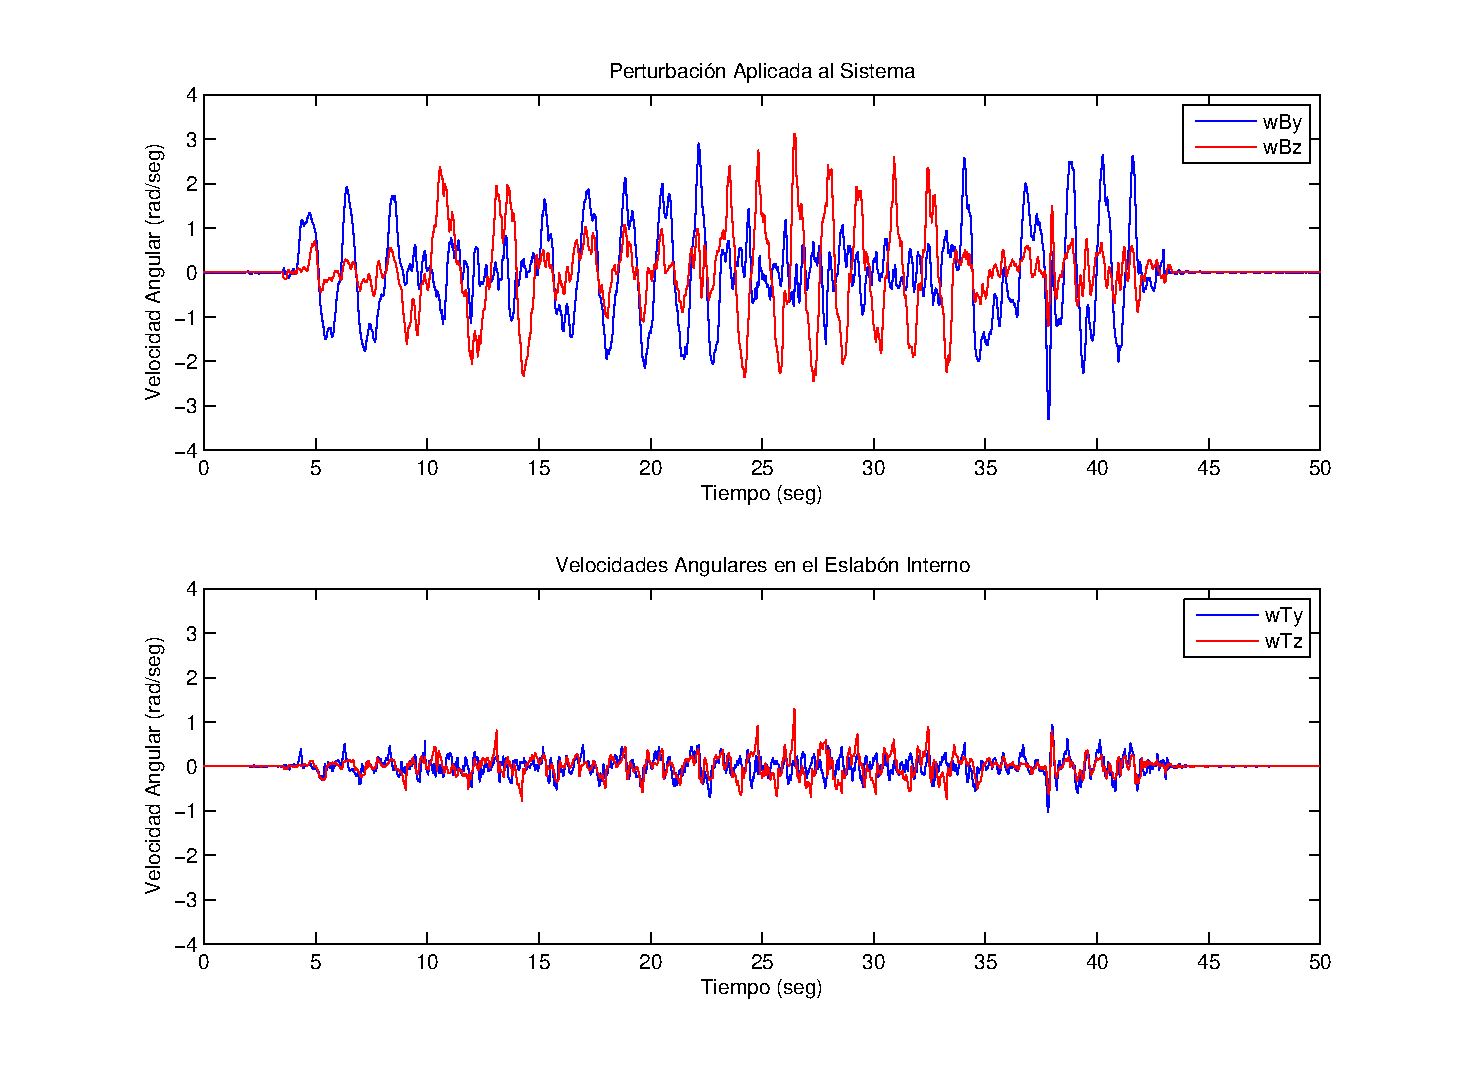
\includegraphics[scale=0.63,trim = 20mm 0mm 20mm 0mm]{img/ResSMPer.eps}
%trim = izquierda abajo derecha arriba [scale=0.5,trim = 40mm 30mm 110mm 15mm, clip]
      \caption{Resultados de la Estabilizaci\'{o}n por Modos deslizantes}
      \label{fig:ResSMPer}
\end{figure}

Es evidente que el control por modos deslizantes tiene un mejor desmpe\~{n}o que el compensador proporcional-integral, pues cancela de una mejor manera las perturbaciones. En la figura ~\ref{fig:ResSMVs}-a se muestra la gr\'{a}fica de la perturbaci\'{o}n en el eje-$y$ contra la velocidad angular medida en el eje de elevaci\'{o}n, mientras que en la figura ~\ref{fig:ResSMVs}-b se muestra la perturbaci\'{o}n en el eje-$z$ graficada junto con la respuesta del sistema en el eje de elevaci\'{o}n cruzada. 

\begin{figure}[H]
\centering 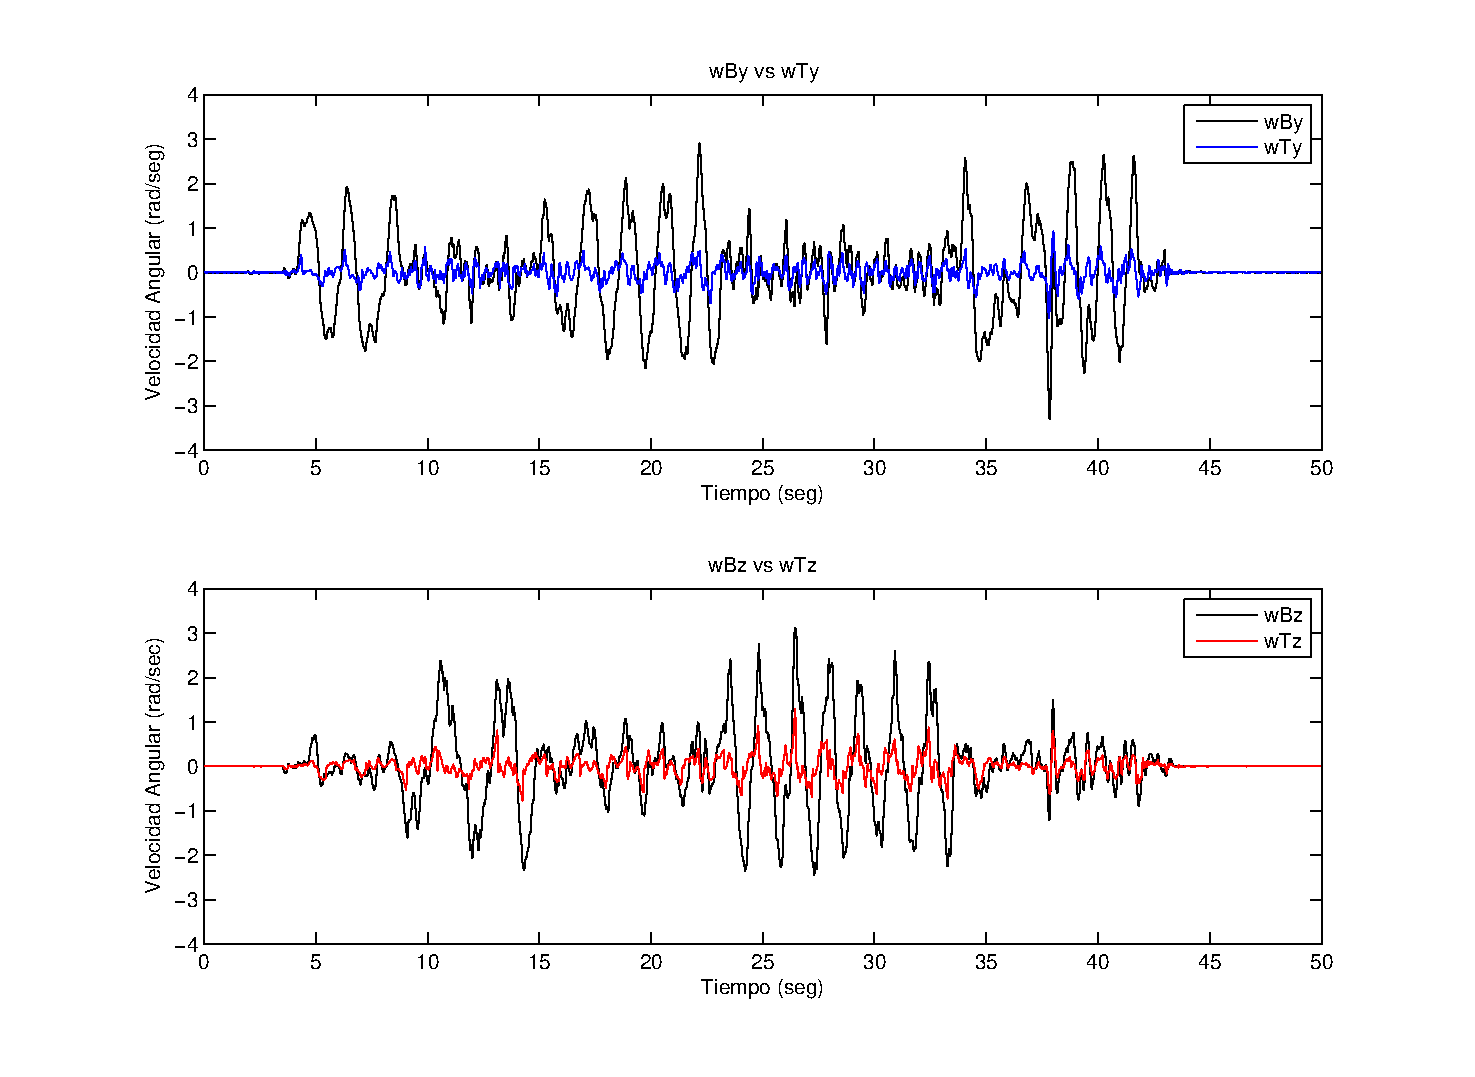
\includegraphics[scale=0.63,trim = 20mm 0mm 20mm 0mm]{img/ResSMVs.eps}
%trim = izquierda abajo derecha arriba [scale=0.5,trim = 40mm 30mm 110mm 15mm, clip]
      \caption{Resultados de la Estabilizaci\'{o}n por Modos deslizantes}
      \label{fig:ResSMVs}
\end{figure}

Haciendo una comparativa entre las perturbaciones y las respuestas de cada algoritmo implementado podemos concluir que el algoritmo de estabilizaci\'{o}n por modos deslizantes tiene un mejor desempe\~{o} que el compensador PI pues su respuesta presenta un menor error en la cancelaci\'{o}n de la perturbaci\'{o}n, es decir, mantiene la velocidad angular en el eje de elevaci\'{o}n y elevaci\'{o}n cruzada m\'{a}s cercanas al cero, adem\'{a}s de haber compensado mejor una perturbaci\'{o}n de una frecuencia ligeramente mayor.  